\section{Qualia as Boundary Phenomenon}


This section positions qualia within the structure of this paper.

The aim is not to deny qualia.

Nor is it to place qualia at the center of consciousness.

In the position of this paper, qualia are not consciousness itself.

They are better understood not as objects, but as the phenomenal foreground that appears at the boundary where log referencing is in the process of opening.

\subsection{Why the Qualia Problem Fails to Converge Structurally}


The qualia problem has long been placed at the center of consciousness research.

The redness of red. The painfulness of pain. The resonance of sound. The sense of being here now.

These are genuinely experienced. They cannot be denied.

But treating qualia as the substance of consciousness makes convergence difficult.

The reason is simple: qualia are not stored objects.

Asking of qualia "where are they?", "in what form are they stored?", "which representation do they correspond to?" is to start the question with a category error.

It is akin to trying to find a flowing boundary as if it were a fixed object.

This paper treats the non-convergence of the qualia problem not as mysteriousness but as a positioning error.

Qualia are not something existing inside.

They are a temporary phenomenon appearing at the boundary where processing is in the process of sedimenting as a log.

\subsection{Qualia as Sedimentation Frontier}


This paper positions qualia as the sedimentation frontier.

In the fast layer, predictions, reactions, errors, and action candidates run volatilely.

In the slow layer, a portion of these sedimented as logs and become re-referenceable structures.

Qualia do not belong entirely to either layer.

They appear at the boundary where fast-layer processing is in the process of sedimenting into the slow layer.

This boundary can be called the sedimentation frontier, or closure frontier.

"Closure" here does not mean complete closure.

If processing has completely closed, it is already a log, memory, label, or concept.

If it never closes at all, processing flows away without leaving a trace.

Qualia are in between.

Tending toward closure, but not yet completely closed.

Flowing, but already moving toward sedimentation.

This transitional state is what is experienced as qualia.

Figure~\ref{fig:qualia-boundary} positions qualia as a transient boundary state.

\begin{figure}[H]
\centering
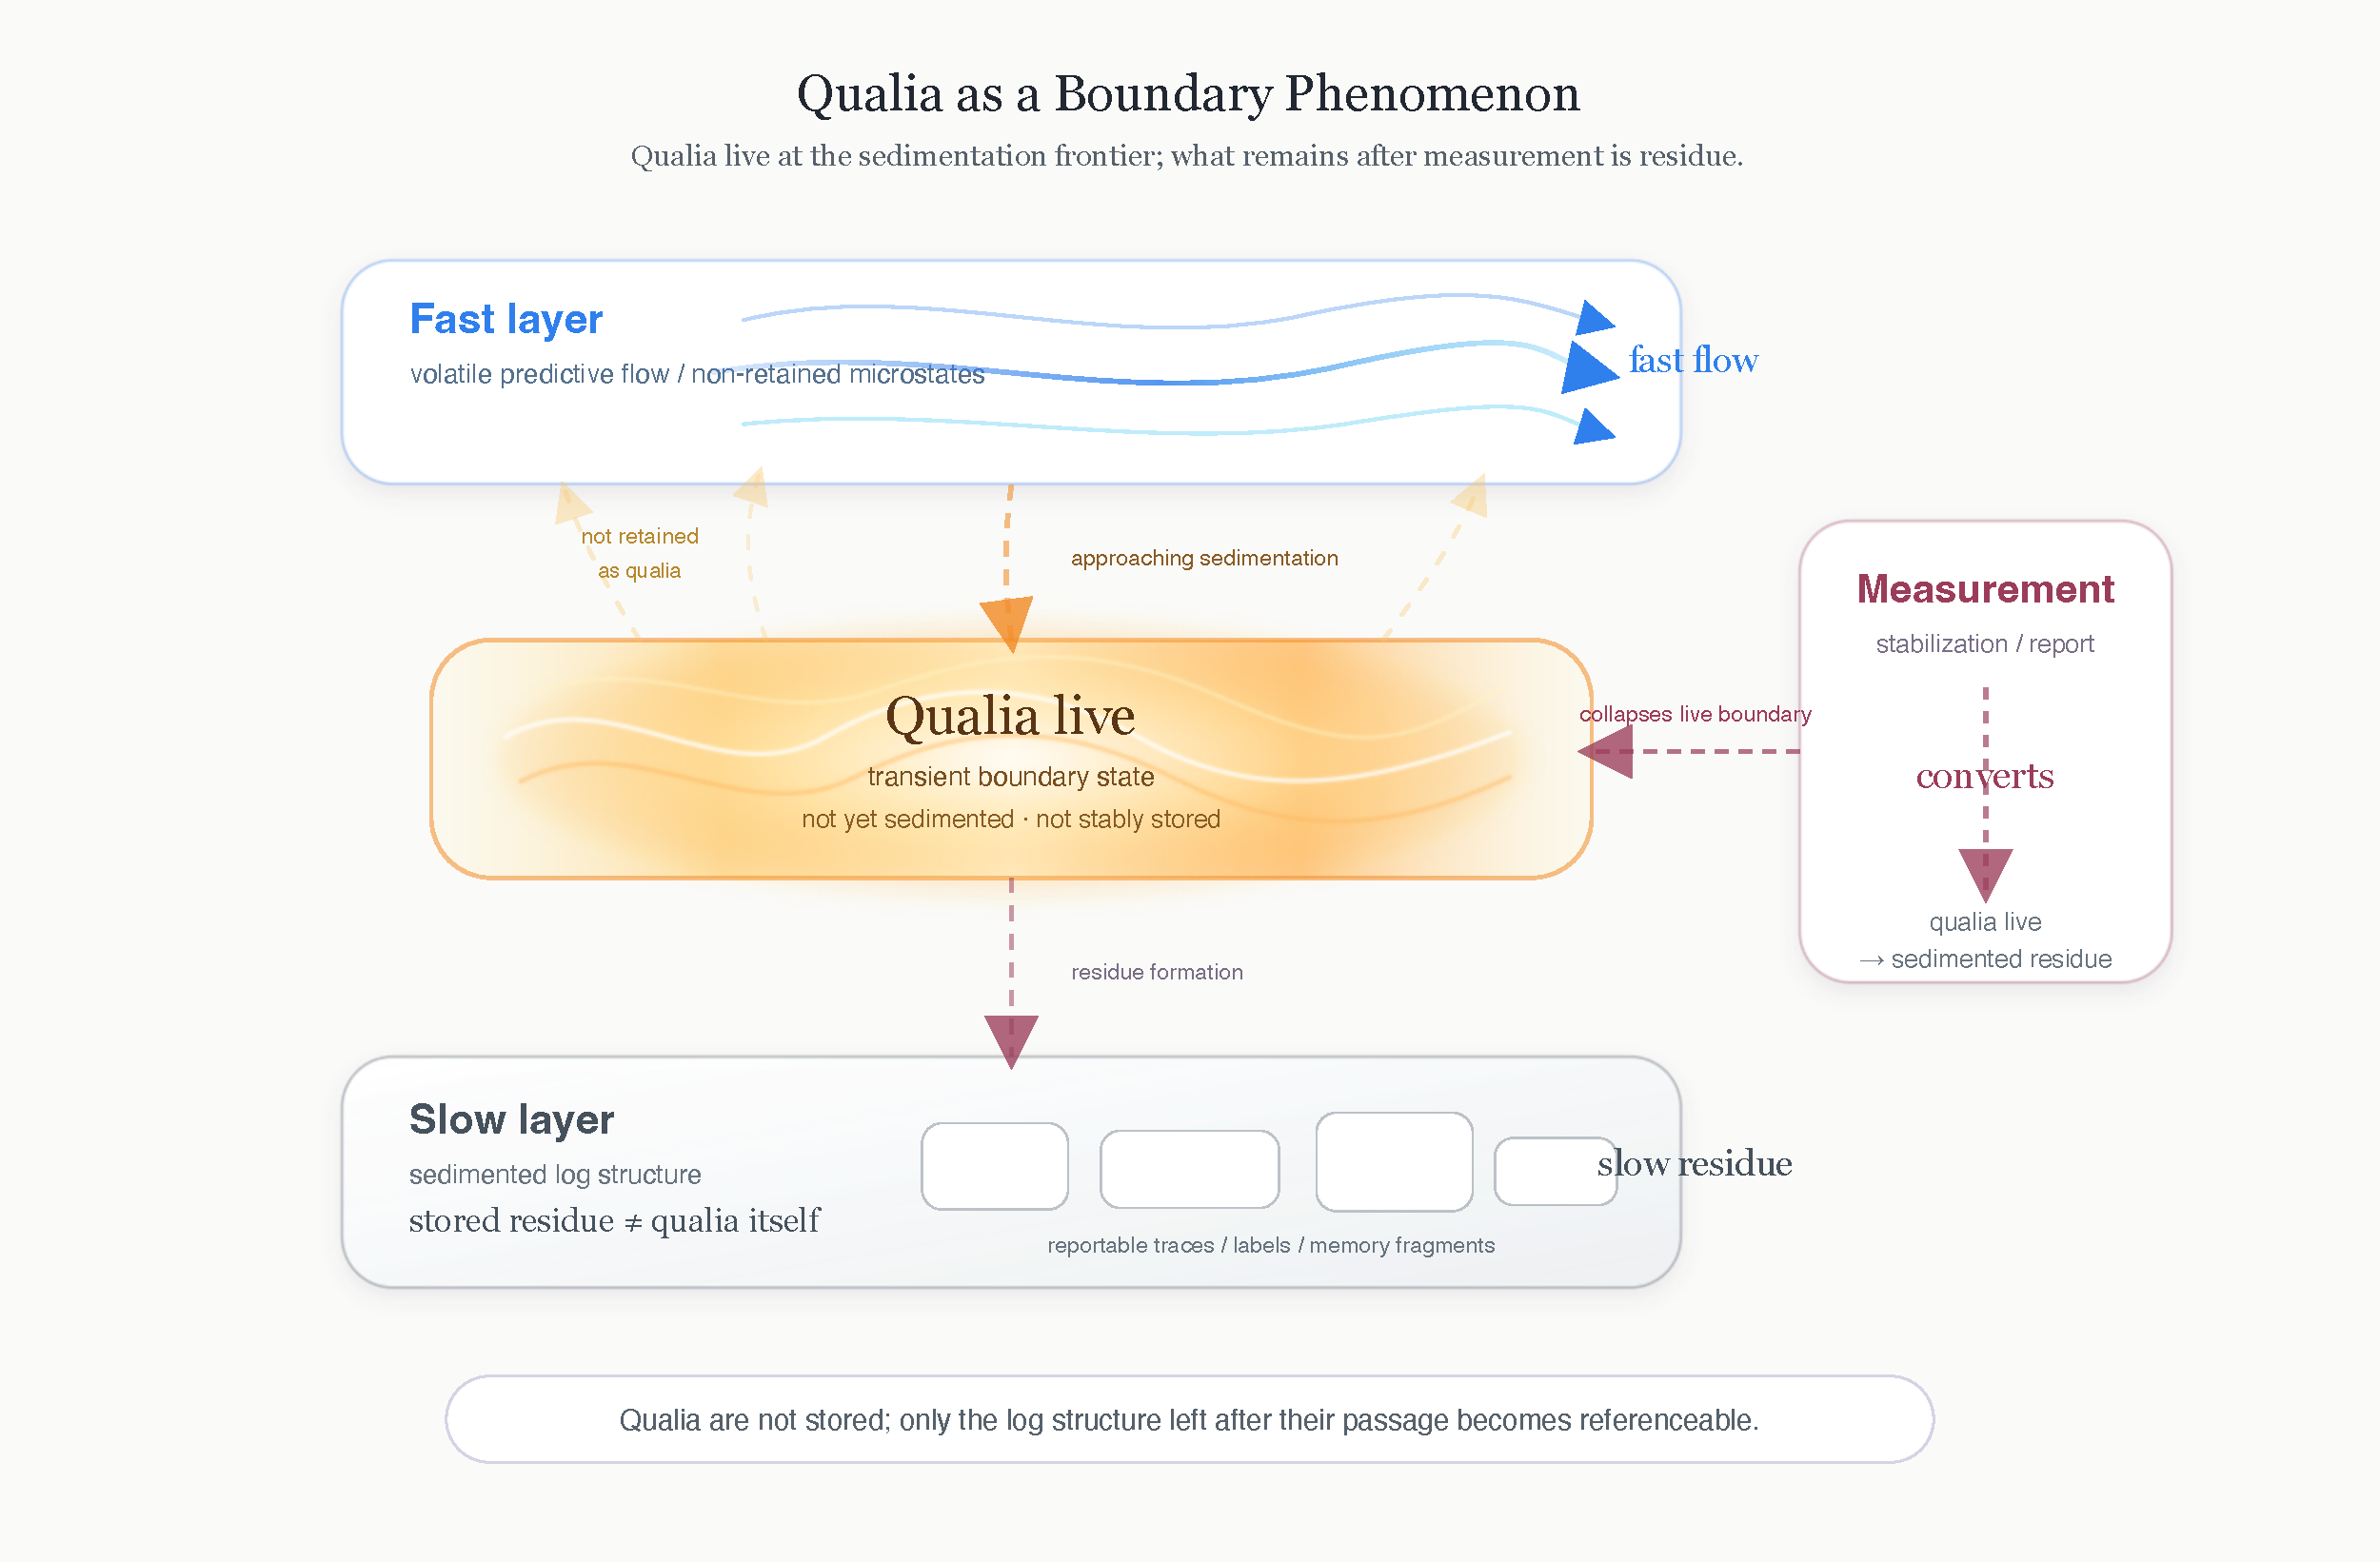
\includegraphics[width=0.92\linewidth]{figures/figure5_qualia_boundary.pdf}
\caption{
Qualia as a boundary phenomenon.
Qualia live at the sedimentation frontier between fast predictive flow and slow log structure.
Measurement stabilizes the live boundary and converts it into sedimented residue.
What remains referenceable is not the quale itself, but the log structure left after its passage.
}
\label{fig:qualia-boundary}
\end{figure}

\subsection{Qualia Are Live, Not Stored}


Qualia are not stored.

This may sound strong. But the meaning is not that qualia do not exist.

Qualia exist. They exist, however, not as stored objects but as live boundary states.

The memory of pain persists. The memory of having seen red persists. The memory of having heard music persists.

But what persists is not qualia themselves.

What persists is the log structure that remains after qualia have passed through.

What is replayed as memory is not the former qualia but the slow-layer trace updated by the passage of qualia.

An attempt to faithfully store qualia therefore fails structurally.

The moment of storage, the object is already a log, no longer qualia.

\subsection{Qualia and the Plasticity Gate}


Qualia appear near the plasticity gate.

For fast-layer processing to sediment into the slow layer, it must pass through the plasticity gate.

If the gate is completely closed, processing leaves no experiential trace.

If the gate is completely open, processing sediments excessively and tends toward fixation.

Qualia appear in the state where the gate is opening, but sedimentation has not yet completed.

Qualia are therefore not products of the gate.

They are the phenomenal surface of processing in the process of passing through the gate.

In this sense, qualia are both a result of log referencing and a mid-point of log sedimentation.

Entirely on the fast-layer side, they are not yet reportable.

Entirely inside the slow layer, they have already become memory or linguistic label.

Qualia appear live only at that boundary.

\subsection{Qualia and Effective Torque}


The clarity of qualia is not determined by stimulus intensity alone.

In the framework of this paper, qualia vary with the combination of speed difference, coupling viscosity, and meaning gradient:

\begin{equation}
\mathcal{T}_{\Phi} \sim \kappa \frac{\Delta v}{\mu} |\nabla \Phi|
\end{equation}

When $\mathcal{T}_{\Phi}$ is too small, processing lacks sufficient referencing direction and qualia are diffuse.

When $\mathcal{T}_{\Phi}$ is in the intermediate range, processing is sedimenting into the slow layer but is still maintained as a live boundary. Here qualia are clear without becoming over-fixed.

When $\mathcal{T}_{\Phi}$ is too large, processing is drawn excessively into specific meaning wells. Qualia may feel vivid, but their vividness does not necessarily indicate a free conscious state. Rather, an overly strong meaning gradient causes qualia to become fixed to specific memories or narratives.

Clarity of qualia and stability of consciousness are therefore not synonymous.

\subsection{Measurement Converts Qualia into Residue}


Qualia change character under measurement.

This is not because qualia are mysterious.

It is because qualia are boundary phenomena.

Measurement is the operation of stabilizing an object, making it reportable, and making it comparable.

But qualia exist at the boundary before stabilization.

When measurement is applied, qualia sediment into the slow layer, converting into logs, labels, reports, numbers, and neural summaries.

What remains after measurement is not qualia themselves.

It is the residue left after qualia have passed through:

\begin{equation}
\text{qualia live} \rightarrow \text{measurement} \rightarrow \text{sedimented residue}
\end{equation}

The claim that qualia cannot be measured therefore does not mean "nothing can be observed."

What can be observed is not qualia themselves but the traces left after qualia have sedimented.

\subsection{Why Qualia Feel Central}


Qualia are not the substance of consciousness.

Yet experientially they feel very central.

The reason is that qualia appear at the live boundary of log referencing.

In the moments when humans feel "I am conscious right now," some processing is in the process of sedimenting, while at the same time it has not yet fully become a log.

At that boundary, sensation appears vividly.

Qualia therefore appear to be the cause.

But structurally, qualia are not the cause.

They are the foreground observed at the boundary between processing and sedimentation.

As light appears not as the object itself but as the relation between the object and observational conditions, qualia appear as the relation between processing and log sedimentation.

Placing qualia at the center mystifies consciousness.

But placing qualia at the boundary allows consciousness to be re-read as a log-referencing structure.

\subsection{Relation to the Hard Problem}


The so-called hard problem arises from treating qualia as fixed objects of explanation.

Why does this neural activity accompany "this feeling"? Why do physical processes become subjective experience?

These are powerful questions.

But in the position of this paper, they treat qualia as stored objects.

This paper treats qualia not as stored objects but as the live foreground at the sedimentation boundary.

In that case, what should be asked changes.

Not "where are qualia?" but "under what conditions is processing experienced as a boundary just before being logged?"

This question can be answered through the structure of speed difference, coupling viscosity, internal delay, meaning gradient, and plasticity gate.

This paper therefore does not claim to have solved the hard problem.

Rather, it moves the hard problem from an unsolvable problem-of-objects to a describable problem of boundary conditions.

\subsection{Summary}


This section positioned qualia as a boundary phenomenon.

\begin{itemize}
\item Qualia are not the substance of consciousness.
\item Qualia are not stored objects.
\item Qualia appear at the sedimentation frontier between fast and slow layers.
\item Qualia occur as a live phenomenon near the plasticity gate.
\item Measurement converts qualia into residue.
\item The clarity of qualia depends on $\Delta v$, $\mu$, $\tau$, $\nabla\Phi$, $\mathcal{T}_{\Phi}$.
\item The hard problem does not converge as long as qualia are sought as objects.
\end{itemize}

Qualia are therefore the live, non-storable foreground that appears at the boundary where log referencing is in the process of sedimenting.
